%%%%%%%%%%%%%%%%%%%%%%%%%%%%%%%%%%%%%%%%%
% Professional Formal Letter
% LaTeX Template
% Version 2.0 (12/2/17)
%
% This template originates from:
% http://www.LaTeXTemplates.com
%
% Authors:
% Brian Moses
% Vel (vel@LaTeXTemplates.com)
%
% License:
% CC BY-NC-SA 3.0 (http://creativecommons.org/licenses/by-nc-sa/3.0/)
%
%%%%%%%%%%%%%%%%%%%%%%%%%%%%%%%%%%%%%%%%%

%----------------------------------------------------------------------------------------
%	PACKAGES AND OTHER DOCUMENT CONFIGURATIONS
%----------------------------------------------------------------------------------------

\documentclass[12pt, a4paper]{letter} % Set the font size (10pt, 11pt and 12pt) and paper size (letterpaper, a4paper, etc)

\input{structure.tex} % Include the file that specifies the document structure

\newcommand{\bibsection}[1]{}
\newcommand{\section}[1]{}
\newcommand{\newblock}{}

\newenvironment{thebibliography}[1]%
      {References\begin{description}}{\end{description}}
   \newcommand{\htmlbibitem}[2]{\label{#2}\item[{[#1]}]}
\usepackage[authoryear]{natbib}

\newenvironment{reply}{$\triangleright$\bf}{$\triangleleft$}
\renewenvironment{quote}
               {\list{}{\rightmargin\leftmargin}%
                \item\relax\normalfont}
               {\endlist}

\setlength\parskip{\bigskipamount} \setlength\parindent{0pt}

%\longindentation=0pt % Un-commenting this line will push the closing "Sincerely," and date to the left of the page

%----------------------------------------------------------------------------------------
%	YOUR INFORMATION
%----------------------------------------------------------------------------------------


\Who{Dr. Luiz Max de Carvalho} % Your name

\Title{, PhD} % Your title, leave blank for no title
\authordetails{
	School of Applied Mathematics\\ % Your department/institution
	Praia de Botafogo, 190\\ % Your address
	Rio de Janeiro, RJ, 22250-900\\ % Your city, zip code, country, etc
	Email: lmax.fgv@gmail.com \\ % Your email address
	Phone: +55 21 3799-2348 \\ % Your phone number
% 	URL: LaTeXTemplates.com % Your URL
}

%----------------------------------------------------------------------------------------
%	HEADER CONTENTS
%----------------------------------------------------------------------------------------
\logo{emap.png}
% \logo{Marca_FGV_EMAp_colorida.png}

\headerlinetwo{Getúlio Vargas Foundation (FGV)} % Top header line, leave blank if you only want the bottom line

% \headerlinetwo{School of Applied Mathematics (EMAp)} % Bottom header line

%----------------------------------------------------------------------------------------

\begin{document}

\documentclass[10pt]{article}
\usepackage{amsmath}
\usepackage{amssymb}
\usepackage{graphicx}
\usepackage{color} % for revision purposes only, may be not present in the final file
% cite package, to clean up citations in the main text. Do not remove.
% \usepackage{cite}
\usepackage{color}
\usepackage{indentfirst} %% LM: in order to indent the first paragraph of each section
\usepackage{url} %% LM: in order to include nice urls
\usepackage{booktabs} %% LM: nice tables...
\usepackage{subfigure} % LM: panels
\usepackage[authoryear,round]{natbib}
\bibliographystyle{apalike}
\usepackage{xr} % automatic cross-referencing
\externaldocument{Text_S2}
% Use doublespacing - comment out for single spacing
%\usepackage{setspace}
%\doublespacing

\topmargin 0.0cm
\oddsidemargin 0.5cm
\evensidemargin 0.5cm
\textwidth 16cm
\textheight 21cm

\usepackage[labelfont=bf,labelsep=period,justification=raggedright]{caption}


\makeatletter
\renewcommand{\@biblabel}[1]{\quad#1.}
\makeatother

\renewcommand{\thesubfigure}{(\Alph{subfigure})}
% Leave date blank
\date{}

\pagestyle{myheadings}
%% ** EDIT HERE **

%% ** EDIT HERE **
%% PLEASE INCLUDE ALL MACROS BELOW

%% END MACROS SECTION

% consistent edits between manuscript and rebuttal letter
\input{make-edits}

\begin{document}

% Title must be 150 characters or less
\begin{flushleft}
{\Large
\textbf{Spatio-temporal Dynamics of Foot-and-Mouth Disease Virus in South America}
}
% Insert Author names, affiliations and corresponding author email.
\\
Luiz Max Carvalho$^{1\ast}$,
Nuno Rodrigues Faria$^{2,3}$,
Andres Perez$^{4}$,
Marc A.~Suchard$^{5,6}$,
Philippe Lemey$^{2}$,
Waldemir de Castro Silveira$^{7}$,
Andrew Rambaut$^{1,8,9}$,
Guy Baele$^{2}$
\\
\bf{1} Institute of Evolutionary Biology, University of Edinburgh, Edinburgh, United Kingdom.\\
\bf{2} Department of Microbiology and Immunology, Rega Institute -- KU Leuven, Leuven, Belgium.\\
\bf{3} Department of Zoology, University of Oxford, Oxford, United Kingdom.\\
\bf{4} University of Minnesota, Department of Veterinary Population Medicine, College of Veterinary Medicine, Saint Paul, USA.\\
\bf{5} Departments of Biomathematics and Human Genetics, David Geffen School of Medicine at UCLA, University of California, Los Angeles,  United States of America.\\
\bf{6} Department of Biostatistics, UCLA Fielding School of Public Health, University of California, Los Angeles,  United States of America.\\
\bf{7} Research and Development Division, Trimatrix Applied Biotechnology Ltd, Rio de Janerio, Brazil.\\
\bf{8} Fogarty International Center, National Institutes of Health, Bethesda, MD,  United States of America.\\
\bf{9} Centre for Immunology, Infection and Evolution at the University of Edinburgh, Edinburgh, United Kingdom.
$\ast$ E-mail: lm.carvalho@ed.ac.uk
\end{flushleft}
% Please keep the abstract between 250 and 300 words
\section*{Abstract}

\myedit{RefOneComOne}{
Although foot-and-mouth disease virus (FMDV) incidence has decreased in South America over the last years, the pathogen still circulates in the region and the risk of re-emergence in previously FMDV-free areas is a veterinary public health concern.
In this paper we merge epidemiological and genetic data to reconstruct spatiotemporal patterns and determinants of FMDV serotypes A and O dispersal in South America.
}

Key-words: Phylogeography, foot-and-mouth disease virus, South America, animal trade.

\section*{Introduction}

% \myedit{RefOneComOne}{}

Foot-and-mouth disease virus (FMDV) is a rapidly evolving picornavirus and the causative agent of foot-and-mouth disease (FMD), the most important disease of domestic and wild cloven-hoofed animals~\citep{Grubman2004}.
The virus can be classified in seven serotypes, three of which (A, O, and C) have circulated in South America.
Serotype A caused large epidemics throughout the Southern cone in recent years~\citep{Perez2001, Malirat2012}, while endemic circulation has been mostly limited to Venezuela~\citep{Malirat2012}.
Historically, serotype O has been the most prevalent serotype on the continent, but is now limited to areas in the Andean region, and in particular to Ecuador~\citep{Malirat2011a}.
\myedit{RefOneComTwo}{Serotype C on the other hand was last encountered in the continent in $1995$ in Brazil~\citep{Correa2002}.}
Historical reports suggest that FMDV arrived in South America in the late years of the 19th century with European colonization~\citep{Naranjo2013, Tully2008}. 
By the 1970s, FMD was widespread in the region, with several large-scale epidemics being caused by multiple subtypes~\citep{Saraiva2003}.
In South America, FMD control and eradication has traditionally been pursued using a combination of mass vaccination programs~\citep{Saraiva2004b} and control of animal movements from areas in which FMDV infection was suspected.
Over time, passive and active surveillance programs have, with different degrees of success, managed the early detection of FMDV.
In order to achieve complete eradication however, the strains involved in epidemics - especially those in previously FMDV-free areas - need to be accurately characterised.

Phylogenetic analyses have proven useful in recovering the transmission pathways from genetic data~\citep{Cottam2008a, Cottam2008b} and providing insight into the processes that drive re-emergence~\citep{DiNardo2011}.
More recently, molecular epidemiology tools have been used to infer the origin and evolutionary history of emerging strains in South America~\citep{Perez2001, Malirat2007, Malirat2011a, Malirat2011b, Maradei2013}.
However, as pointed out by Di Nardo, Knowles \& Paton~\citep{DiNardo2011}, a common feature of FMDV molecular epidemiology studies is that  joint evaluation of epidemiological, environmental and genetic data has usually been performed outside of an unified quantitative framework.
In the face of many sources of information, ranging from genetic data to environmental data on host distribution and outbreak counts, it's desirable to have a framework capable of integrating these sources of information coherently.
Phylodynamics combines population genetics and epidemiology to explicitly  model the interaction between ecological processes such as migration and selection and the shape of the phylogenies~\citep{Grenfell2004, Volz2013}.
Bayesian phylodynamics offers an attractive statistical framework to combine multiple sources of information while marginalizing over the topology space, thus accommodating phylogenetic uncertainty.
In particular, phylogeographic methods can be employed to understand viral spatial dynamics under explicit spatial diffusion models~\citep{Lemey2009}.
Further, an important research goal is to gain insight into the major determinants of FMDV spread in the continent.
Since animal movements constitute a major threat to eradication programs~\citep{Schley2009}, using animal trade data as predictors can be a valuable tool to understand the role of livestock commerce in the spread of FMDV.
For example, Nelson et al. ~\citep{Nelson2011} coupled swine trade data and genetic data to show that swine movements in the United States drove the spread of a novel influenza virus of the H1 subtype.

Here, we investigate the phylodynamic patterns of serotypes A and O in South America using all publicly available VP1 (1D) sequences for those serotypes in South America, sampled over a long time-period (1955-2010 for serotype A and 1994-2010 for serotype O) in nearly all south American countries affected by FMD.
We apply Bayesian phylogeographic methods to investigate the evolutionary dynamics of serotypes A and O in South America incorporating  genetic, spatial and epidemiological data such as livestock trade, geographic distances and vaccination coverage.
This flexible Bayesian phylogeographic framework allows for the testing of hypotheses concerning viral dispersal, while naturally accommodating phylogenetic uncertainty~\citep{Lemey2009, Faria2011}.
We use BEAST~\citep{Drummond2012} to infer time-structured phylogenies and reconstruct past population dynamics, to which we overlay vaccination and serotype-specific notification data.
To study the factors driving re-emergence, we use data on livestock trade and geographical distances as predictors for viral spatial diffusion and compare competing spatial dynamics models involving each predictor using recently developed methods. 

\section*{Results}

\section*{Discussion}

\subsection*{Sampling bias}
Spatial: sequences included as predictors in various ways in spatial genetic GLM
Temporal: 

\section*{Methods}
\subsection*{Genetic and epidemiological data}

\textbf{Genetic data.}
We retrieved all FMDV nucleotide sequences available from GenBank~\citep{Benson2013} from the National Center for Biotechnology Information (NCBI, \url{ http://www.ncbi.nlm.nih.gov/}) with more than $600$ bp.
This first step yielded $6, 907$ sequences which were then filtered to exclude all sequences that did not include the 1D (VP1) gene, resulting in $4, 507$ sequences being kept.
We then filtered for sequences from serotypes A and O, yielding $1051$ and $2350$ sequences, respectively.
Next, we excluded sequences that had been extensively passaged in cell culture and selected all sequences from South America (Argentina, Bolivia, Brazil, Colombia, Ecuador, Paraguay, Peru, Uruguay, Venezuela) for which information on country and year of isolation was available.

This resulted in $185$ sequences (from eight countries) for serotype A and $215$ sequences (nine countries) for serotype O, covering time spans of $58$ ($1955$-$2013$) and $53$ (1958-2011) years, respectively (see Tables~\ref{stab:sequences_A} and~\ref{stab:sequences_O} for details).
We aligned each data set using the MAFFT~\citep{Katoh2002} algorithm implemented in the Geneious~\citep{Kearse2012} software package.
After a preliminary phylogenetic analysis (see below), an early serotype A sequence (Venezuela 1951) was excluded because its root-to-tip divergences was incompatible with its sampling date~\citep{Rambaut2016}.
For serotype O, five sequences were excluded under the same criteria (Table~\ref{stab:exclseqs}).
The final data sets had $184$ and $210$ sequences for serotypes A and O, respectively.

\textbf{Acquisition of trade data.}
Data on animal trade were obtained from the FAO database (\url{http://faostat.fao.org/}).
We retrieved data on the \textit{detailed trade matrix} for cattle, pigs and sheep (number of live animals exchanged) covering the period from $1986$ to $2009$, for each of the nine countries.

\textbf{Vaccination and case data.}
Data on the number of vaccine doses (irrespective of serotype) from 1990 to 2010 were obtained from the PANAFTOSA annual reports (\url{https://www.paho.org/panaftosa/}) and then standardised to doses per (cattle) head in each country.
Serotype-specific outbreak notifications were obtained from FMD Bioportal (\url{http://fmdbioportal.ucdavis.edu:8080/}).

\textbf{Data availability.} All the data used in this paper including BEAST XML files are hosted at~\url{https://github.com/maxbiostat/FMDV_AMERICA}.


In this study we take a Bayesian approach to testing evolutionary hypotheses while accommodating phylogenetic uncertainty.
Details on computational settings and prior choice can be found in Text S2.
\subsection*{Phylogenetic Analysis}

We assume a general time reversible (GTR)~\citep{Tavare1986} model of sequence evolution, along with gamma-distributed rate heterogeneity (4 categories) for all our analyses.
We conducted an initial analysis of the two data sets described, employing PhyML~\citep{Guindon2003} to obtain maximum likelihood phylogenies which we then used in conjunction with Tempest~\citep{Rambaut2016} to produce root-to-tip divergence (RDV) plots and identify discrepant sequences (see ~\cite{Rambaut2016} for details).

Having identified considerable rate variation among branches we used the Bayesian Evolutionary Analysis by Sampling Trees (BEAST)~\citep{Drummond2012,Suchard2018} software package to infer time-structured phylogenies under relaxed clock models~\citep{Drummond2006}, employing the BEAGLE~\citep{Ayres2012} library to gain computational efficiency.

\subsection*{Model selection}

In order to compare the performance of combinations of sequence evolution (Markov) and relaxed clock models for each data set (see Text S2), we use state-of-the-art marginal likelihood estimators, namely generalised stepping-stone sampling (SS)~\citep{Baele2015} implemented in BEAST~\citep{Suchard2018}.
Following a preliminary Skygrid analysis, we chose the constant population size coalescent parametric model -- and its associated working prior -- as the tree prior for these comparisons.

\subsection*{Spatio-temporal Dynamics}

\textbf{Effective population size reconstruction}.
We employed the Skygrid coalescent model~\citep{Gill2012} to reconstruct that past population dynamics of both serotypes.
Skygrid necessitates the specification of a cutoff value, $K$, commensurate with the age of the root (time to the most recent common ancestor, tMRCA) .
We have used $K = 150$ years for serotype A and $K = 100$ for serotype O sets as conservative estimates of the tMRCA of the sampled sequences. 
In addition, we employed the generalised linear model proposed by~\cite{Gill2016} to test the association between several temporal predictors such as vaccination, overall livestock trade and production in South America and numbers of cases of each serotype, as follows.
These were the total number of live animals produced and traded between the 9 countries considered here for five livestock: cattle, goats, sheep, pigs and horses, totalling 10 predictors.
In addition to these livestock-associated predictors, we also considered the number of vaccine doses per (cattle) head along with its dispersion (see Text S2) and the number of cases for each serotype.
In total there were $13$ temporal predictors for each serotype.
To facilitate computation we divided each predictor by its maximum value so as to bring all predictors to the common scale of $[0, 1]$ (see Text S2 for more details).
%TODO: thinking of presenting a table with rows = predictors and cols = name, temporal_range, { beta (CI) } x serotype

\textbf{Phylogeographic generalised linear models}.

In order to study the influence of different epidemiological predictors on viral diffusion through space, we used information on the trade of live cattle, pigs and sheep divided in three periods ($1986-1995$,~$1996-2004$,~$2005-2013$).
We also included the great circle distance between the (centroids of) countries and the presence/absence of borders between countries as predictors.
Additionally, to assess the influence of sequence (spatial) sampling, we also included the product and absolute differences in sequence (samples) numbers between locations as a predictor of flow (see the appendix in~\cite{Lemey2014} for a discussion).
The numbers of sequences in each location were also included as origin and destination predictors (see~\cite{Dudas2017}), leading to a total of $14$ predictors being considered.
In order to test the relevance of each predictor to spatial spread we used Bayesian stochastic variable selection (BSSVS, \cite{Lemey2009}).
All predictors with the exception of the borders were transformed using $\log(x +1)$ in order to map $0$ to $0$ and standardised to have mean $0$ and standard deviation $1$.
The relevance of each predictor can then be determined using Bayes factors~\citep{KassRaftery1995,Lemey2009,Lemey2014}.
Details are given in Text S2.

\section*{Software versions and computer programs}

\begin{itemize}
 \item \textbf{PhyML} version 3.0, downloaded from~\url{www.atgc-montpellier.fr/phyml/};
 \item \textbf{Tempest} version 1.5.1, downloaded from~\url{http://tree.bio.ed.ac.uk/software/tempest/}  ;
 \item \textbf{BEAST} version 1.10.4, downloaded from~\url{https://github.com/beast-dev/beast-mcmc/releases/download/v1.10.4/};
 \item  \textbf{Jupyter} version 4.4.0, installed from the official Ubuntu repositories;
 \item \textbf{R} version 3.5.0, downloaded from~\url{https://cran.r-project.org/}.
\end{itemize}

All analyses conducted within a GNU/Linux computational environment.
Code to produce many of the plots/analyses is available from~\url{https://github.com/maxbiostat/FMDV_AMERICA}.

\section*{Acknowledgments}
The authors would like to thank Ant\^onio Mendes (PANAFTOSA) for clarifications regarding the vaccination data, Matthew Hall (Oxford), Mandev Gill (Leuven) and Oliver Pybus (Oxford) for insightful contributions and Miguel Carvalho, Felipe Figueiredo (Fiocruz) and Mauricio Oliveira (UFRJ) for operational support.
We acknowledge the support of the National Evolutionary Synthesis Center (NESCent) through a working group (Software for Bayesian Evolutionary Analysis).

\emph{Funding:} The research leading to these results has received funding from the European Union Seventh Framework Programme [FP7/2007-2013] under Grant Agreement no. 278433-PREDEMICS and ERC Grant agreement no. 260864.
This work was also supported by National Institutes of Health grants R01 HG006139 and National Science Foundation grants DMS 1264153.

\emph{Conflict of Interest:} none declared

\newpage
\bibliography{FMDV_AMERICA}
% \newpage
\section*{Figure Legends}
\newpage
\section{Figures and Tables}
%%%%%%%%%%%%%%%%%%%%%%%%%%
%%%%%%%%%%%%%%%%%%%%%%%%%%
% \begin{figure}[!ht]
% \begin{center}
% \subfigure[A]{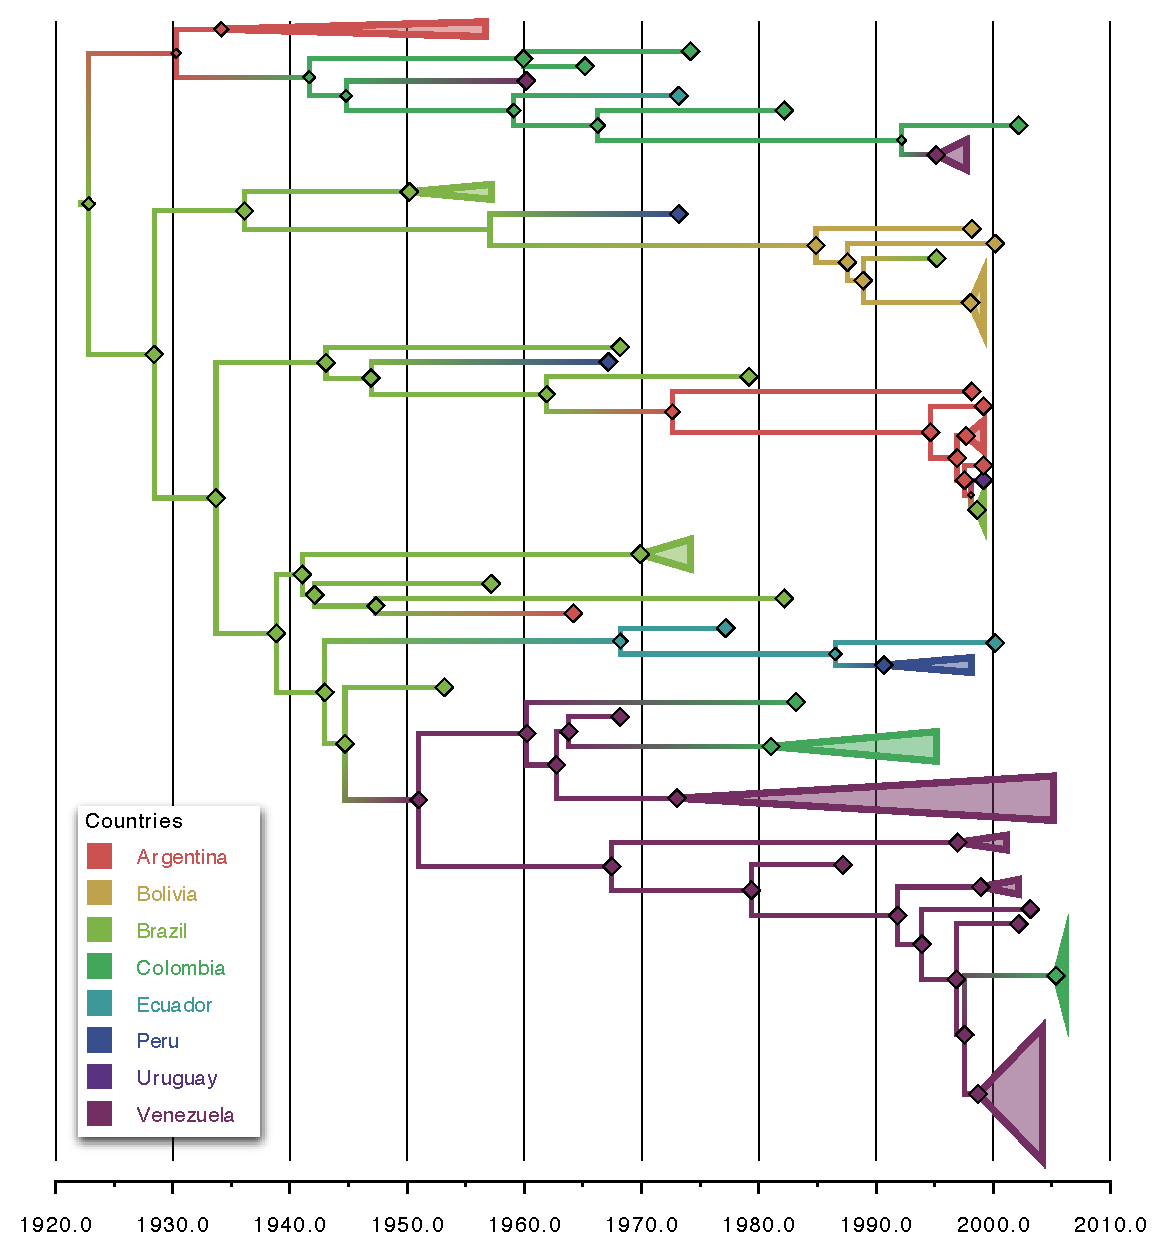
\includegraphics[scale=.45]{FIGURES/A.pdf}}\\
% \subfigure[O]{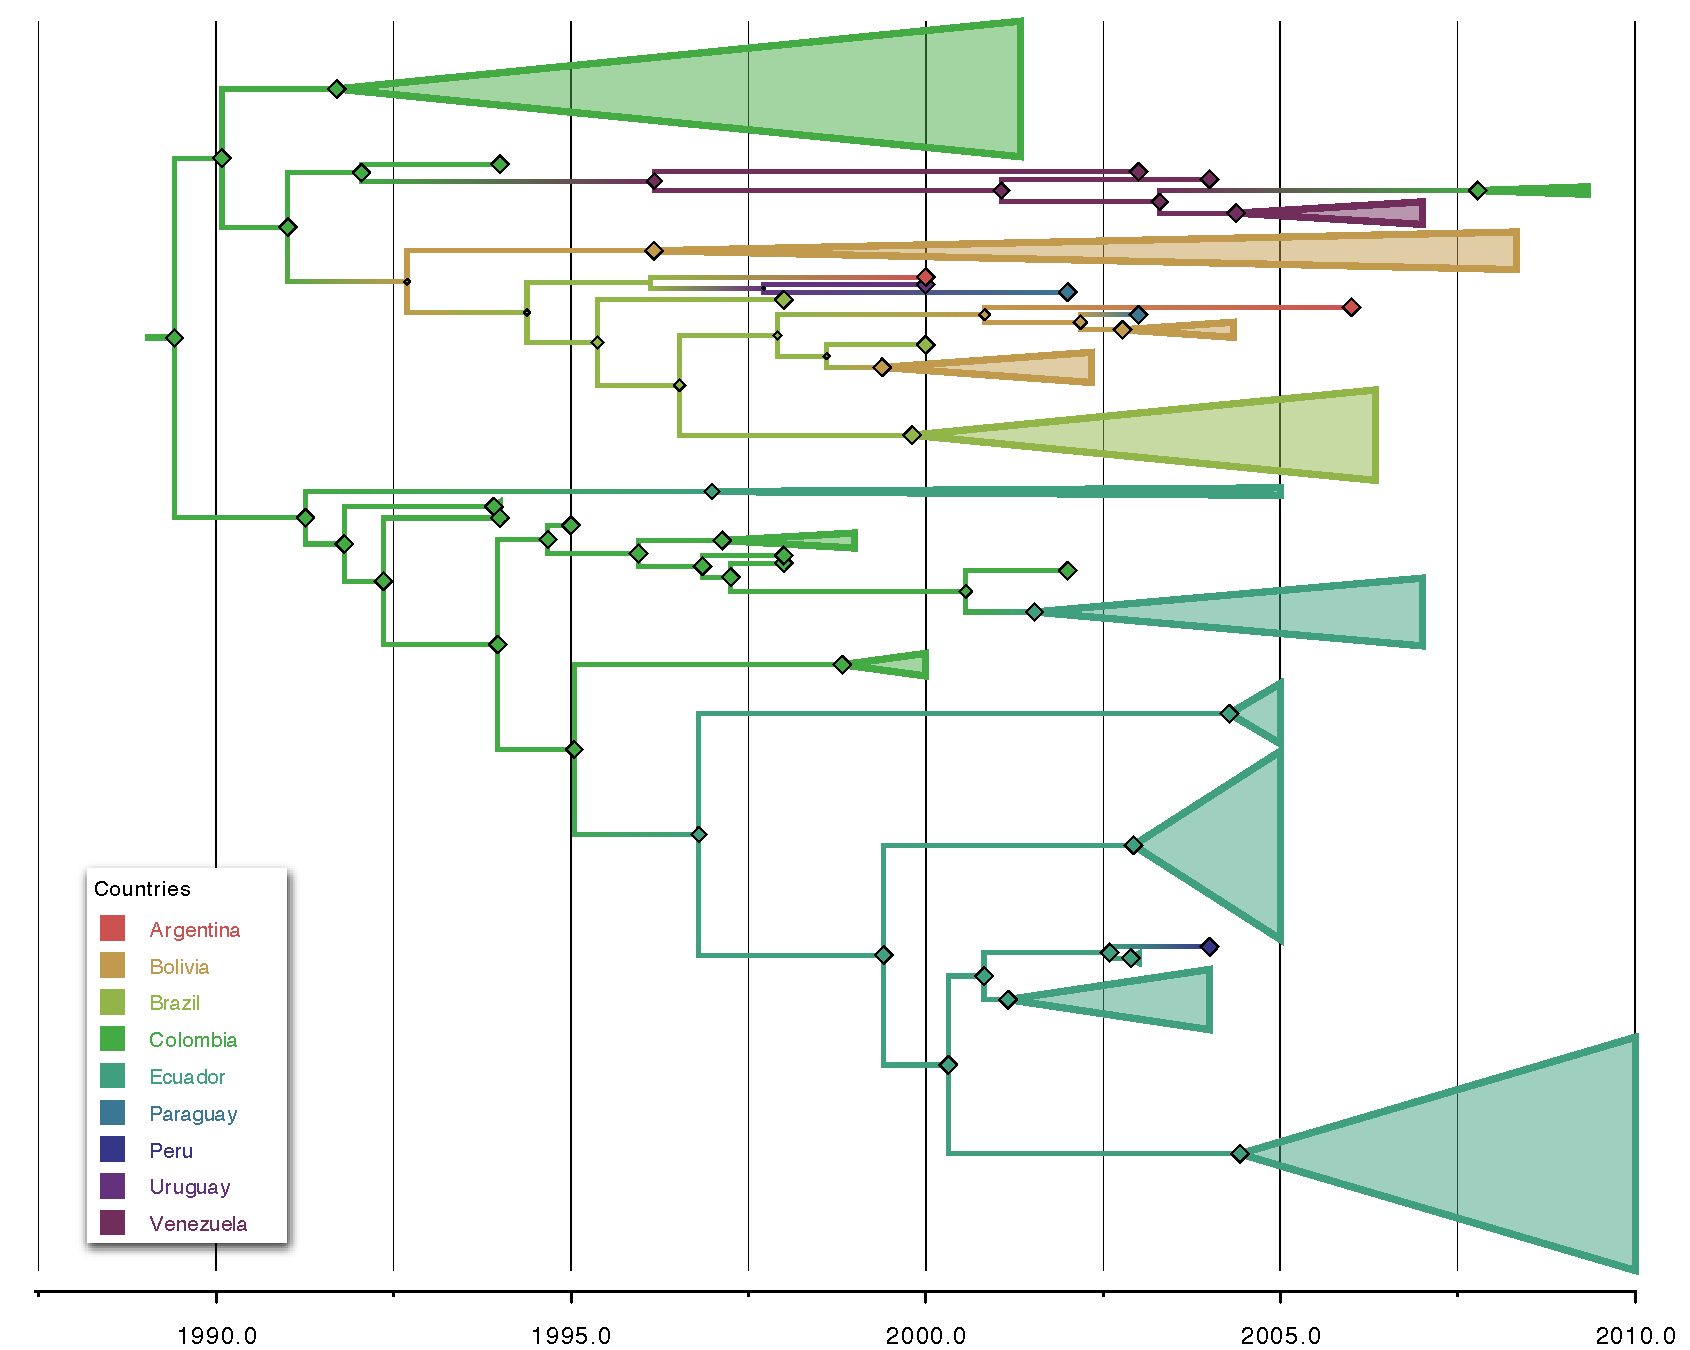
\includegraphics[scale=.30]{FIGURES/O.pdf}}
% \end{center}
% \caption{}
% \label{fig:trees}
% \end{figure}
% %%%%%%%%%%%%%%%%%%%%%%%%%%
% %%%%%%%%%%%%%%%%%%%%%%%%%%
% \begin{table}[H]
% \caption{
% \textbf{.}
% }
% \begin{center}
% \begin{tabular}{lrrrrrr}
% \toprule
%  & \multicolumn{3}{c}{Serotype A}& \multicolumn{3}{c}{Serotype O}\\
%  \midrule
% Predictor & PS & SS & log BF$^2$ & PS & SS & log BF \\
% %\hline
% Cattle&-12588.76&-12591.26&-27.70&\textbf{-8308.94}&\textbf{-8311.21}& \textbf{13.49}\\
% Distance&\textbf{-12557.69}&\textbf{-12559.73}&\textbf{3.83}&-8313.89&-8315.37&9.33\\
% Pigs&-12589.33&-12590.94&-27.38&-8325.39&-8326.63&-1.93\\
% Sheep&-12570.67&-12572.56&-9.00&-8326.23&-8330.64&-5.94\\
% \\
% \hline
% Equal rates &-12561.98&-12563.56&--&-8321.49&-8324.70&--\\
% \bottomrule
% \end{tabular}
% \end{center}
% \begin{flushleft}
% \end{flushleft}
% \label{tab:preds}
%  \end{table}
%%%%%%%%%%%%%%%%%%%%%%%%
\end{document}
 

\bibliographystyle{mbe}

\begin{letter}{
	Dr. Santiago F. Elena\\
    Editor-in-Chief \\
    Virus Evolution
}

%----------------------------------------------------------------------------------------
%	LETTER CONTENT
%----------------------------------------------------------------------------------------

\opening{Dear Dr.~Elena,}

We would like to thank you for the opportunity to re-submit our revised manuscript entitled ``Spatio-temporal Dynamics of Foot-and-Mouth Disease Virus in South America" for consideration for publication in \textit{Virus Evolution}.

In providing our revision, we have carefully considered the helpful suggestions and critiques of yourself and three Reviewers.
You will find a point-by-point response (bold) to all comments (normal text) we received.
Significant changes to the manuscript find themselves in quotes.

\closing{Sincerely,}

\clearpage

% \textbf{General comment \#1: Data corrections}

% \begin{reply}
% \begin{quote}
% \end{quote}
% \end{reply}


%====================
\textbf{Reviewer \#1}
%====================

The authors used sequence data from GenBank to investigate the evolutionary and population dynamics of FMDV serotypes A and O in South America.
They also used utilized a generalized linear model approach to assess the factors contributing to the spread of this virus on the continent.
This involved the incorporation of  the sequence data along with select spatial and epidemiological data to act as proxies for distance and trade and account for possible sampling bias.

Despite the lack of original sequences, the amount and the quality of work done makes this manuscript worth publishing.
The authors have done good job of demonstrating the utility of the GLM approach, even in the absence of temporal sequence data for some countries.
Additionally, the incorporation of the previous reviewers comments has made the manuscript more robust.

I do have some minor comments.

\begin{itemize}
 \item P3 ln3 – You describe the MCC trees for serotype A and O, but these trees show no posterior probability estimates for the internal nodes.
 As this can change the definition of the clades discussed, the statistical support should be included.
 \item P4 ln51 – You make assumptions about the predictors influencing spread, even though the inclusion probabilities are well below 0.25 (except for Pig trade from the serotype A dataset), and BF < 3.
 What is your rationale?
 \item P5 ln13 – Maybe the figure you refer to should be moved to the main manuscript for ease of reading.
 \item P5 ln26 – More oscillations in the genetic diversity are observed for serotype O when the naïve model is used, but the BCI are so wide that these oscillations observed before 1990 (figure 2) are not worth mentioning.
\end{itemize}

%====================
\textbf{Reviewer \#2}
%====================

The authors describe the spatio-temporal dynamics of foot-and-mouth disease (FMD) virus in
South America. They have updated a previous submission of the manuscript as suggested by three referees. The methods used are appropriate and the analyses are reasonable. However, I question the accuracy and choice of some of the sequence data (or its annotation).

Specific points

Page 17, line 54-55: Serotype C was last reported in Amazonas, Brazil in 2004, not in 1995 (Correa Melo, 2004).

Page 18, lines 6-7: The introduction of FMD can be more specifically dated to 1870 in Argentina and chile in 1871 (Machado, 1969).

Page 18, line 42: The time period studied is should be 1955-2013 for serotype A and 1939-2011 for serotype O (see my comments on the sequences available).

Page 20, line 19: “FDMV” should be “FMDV”.

Page 22, lines 48-49: The authors state that “Next, we excluded sequences that had been extensively passaged in cell culture…”. Since passage histories are generally not reported, how was this done? Which sequences were excluded?

Page 22, line 53: “1951-2013” should be “1955-2013”.

Page 23, line 6: “an early serotype A sequence (Venezuela 1951) was excluded because its root-to-tip divergence was incompatible with its sampling date”; this should be type O and not type A.
The sequence in question (AY593827) is probably mis-labelled (and incorrectly dated as 1971 by the original authors) as it is closely related to an Italian virus from 1946.
A better choice would be O3/Venezuela/1951 (AJ004645).

Tables S3 and S4: These table contain inaccuracies and don’t show enough detail to be informative to the reader. I have attached expanded and corrected tables in the form of two Excel spreadsheets (one of each serotype).
This more complete data can be used in the supplementary table.
Inaccuracies have been highlighted in yellow.
There are many cases (mainly in type A) where two or more sequences are of the same strain; I have used strikeout to indicate those that should be removed from the analyses.
Some complete genome sequences reported by Carrillo et al. (2005) are problematic in that the metadata (particularly dates of collection) are incorrect.
Some are even mis-labelled, eg. A18/Zulia/Ven/62 is actually A13/Santos/Bra/58; A32/Venezuela/70 is actually A29/Peru/69.

The sequence of O1/Caseros/ARG/67 (AY593821) is different from other sequences of the same strain (i.e. M89900 \& U82271). One of the latter sequences should be used.
The following sequences could be used to provide earlier examples of South American type O viruses: O/Argentina/1939 (AY593825), O3/Venezuela/1951 (AJ004645), O1/Caseros/Arg/1967 (Caseros, Santa Fé) (M89900 or U82271).
Carrillo et al. (2005) name O/Argentina/1939 as O1 Valle Argentina/39 but report the date as 1953 (probably when it was received at Plum Island).

References

Correa Melo, E. (2004) ‘Outbreaks of FMD type C in Amazonas, Brazil’. In: EMPRES Transboundary Animal Disease Bulletin No 26. Food and Agriculture Organization of the United Nations (FAO): Rome, Italy. http://www.fao.org/3/y5754e03.htm.

Machado, Manuel A. Jr. (1969) AFTOSA: A Historical Survey of Foot-and-Mouth Disease and Inter-American Relations. Albany: State University of New York Press.

Other notes:

1)      FMD type O was introduced into Venezuela in 1950 and was suspected to have originated from the Southern Cone area. FMD type A was introduced into Colombia/Venezuela in 1951 from Europe during a large epidemic of the A5 subtype which also spread to Canada (Saskatchewan in November 1951). It may be useful to include a representative of this epidemic, e.g. A5/Westerwald/West Germany/1951 (AY593781).
This probably gave rise to the later-described A27 subtype in Colombia.
I have provided a map showing the first known occurrences of FMD in the America (PowerPoint file).

2)      A10/Argentina/1961 was from an outbreak linked to a laboratory strain (A10/Holland/1942). The authors are correct in not using this sequence.

3)      A30/Cerro Largo/Uruguay/1950 is sometimes called A Pando or A/8188/69 or A/8188/68. The sequence described by Carrillo et al., 2005 (AY593801) and identified as A30 Uruguay/68 is a sequence from the 2001 outbreak in Uruguay. The genome sequence of AY593801 is identical to AY593802 (identified as A/Uruguay/2001 by Carrillo et al.).

4)      South American vaccine strains (e.g. O1/Campos/Brazil/1958) have probably been reintroduced into the field (either as improperly inactivated vaccines or laboratory escapes) on a number of occasions and have also spread to Europe, particularly during the 1960’s (e.g. UK 1967).

5)      O/BOL/17/90 is a misinterpretation (by the sequence authors) of the WRLFMD sample O/BOL/A/90.


%====================
\textbf{Reviewer \#3}
%====================

The manuscript of Carvalho et al. reports on phylogenetics of foot-and-mouth disease in South America by analysing sequences encoding the VP1 genome region of type O and A FMDV strains circulated in the continent.
This is the second submission to Virus Evolution which I have been invited to review, following the editorial decision of ‘major revision’ to the initial submission with extensive modifications and re-analysis of expanded (omitted) data requested by the reviewers.
The main problems reported by assessing the former submission were concerning: (i) the surprising omission of some VP1 sequences from GenBank that predate the sequence data analysed (and I would stress that this is a study entirely done using sequences retrieved from GenBank), which were absolutely critical to be included in order to have more robust and accurate results, given that the aim of the study was to ‘describe the full history of FMDV in South America’; (ii) in addition to (i), the structure of the dataset analysed was oddly biased in term of time, space and epidemiological setting, which undeniably affected the results of the analyses that were generated using methods that are well-known to  have problem with sampling bias; (iii) how the topics of the study was introduced (i.e. FMD), the review of FMD in South America, selection of the data, and discussion of the (biased) results all revealed a significant lack of knowledge about the history and epidemiology of FMD in South America, which clearly was very unfortunate given the aim of this retrospective study was to provide ‘new insights’ on the epidemiological dynamics of FMD in South America.

This review pertains to the new manuscript submission, but it further assesses the point-by-point responses from the authors to the revisions requested by the reviewers for the initial submission of the manuscript.
I noted that between the first and this submission, some authors abandoned this study and others joined, with the addition of Guido Konig, an expert of FMD.
I very much appreciated and welcome the efforts given by the authors to deal with the issues identified at that time (and as detailed above) by me and the other reviewers.
I also welcome the new methodological approach used to analyse the sequence data, which better addresses sampling biases present in the structure of the data, albeit the one related to the temporal structure sensu strictu.
However, I am still considering the claim on the results provided very weak and only marginally substantiated by using the new analytical approach.
It might be a rather simple and highly subjective opinion, but it seems to me that this study is more a showcase (a word that the authors refer throughout the text when referring to the application of their analytical approach) of analytical methodologies rather than a real focus on FMD dynamics in South America, an opportunity that in my opinion is missed.
This is the message that is conveyed throughout the manuscript and that is sent to the reader, whilst the retrospective investigation of FMD in South America is somewhat lost.
As it seems, the manuscript is structured with a very unbalanced ratio between the writing of FMD-related areas (i.e. review and appraisal of the South America historical data, presentation of the results with an eye on what these would really mean in terms of epidemiological drives and potentially patterns of transmission) and the description of the new methodologies and their properties.
If the target audience of the study would only be readers specifically interested on the methodological approach, the manuscript would be completely fine as it stands.
However, I believe that the main audience would be FMD researchers who might (or more likely not) be very acquainted with mathematical methods or complex analytical approaches.
Engaging the reader with a non-technical style, and resisting the urge to dilute and distract few key messages with other conjecture and the more insipid analyses would be appreciated.

The use of the BNPR-PS model which account for preferential sampling bias in the sequence data is surely providing more robust estimates of Net than a single Skygrid analysis.
However, most of the analsysis the authors have done on this regard is not necessary, considering that the aim of this study is a simple retrospective study on FMD in South America with structurally biased data and not a proof-of-concept for some new methodological approach (something would be very much fit for studies like the Karcher et al., 2016 or Karcher et al. 2020 – when it will be published).
Therefore, the simulation analyses and the corresponding results should be removed from this study. Presenting these results would not be beneficial (if only marginally) and probably of very little interest for the FMD community.
As a matter of fact, references of these results in the main text is only very little and of no relevance.

Using a phylogeographic GLM approach does not make DTA analyses more robust in term or sampling bias, which is clearly what De Maio et al. (2015) and others groups demonstrated.
Phylogeograhic GLM is perfectly valid to test the hypothesis that covariates might (or might not) affect transmission, but it would not derive unbiased results when the structure of the data used for the analysis is inherently biased.
Figure S1 in the Supplementary Information clearly informs on how some country and year of sampling are more represented than others for each of the type O or A data.
As already extensively discussed in the previous review: a proportion of 0.51 type A sequences are form Argentina (75\% of these belonging to a single epidemic), whilst 0.18 are from Venezuela with the majority dated 2002 and later; for type O, a proportion of 0.45 of all sequences are from Ecuador starting from 2002, with 0.18 from Colombia collected before 2002.
So, ~70 of type A sequences are from Argentina and Venezuela, ~64\% of type O from Ecuador and Colombia. From the GLM results it seems that only one single predictor is significantly assessed as driver of transmission for both type O and A, which seems a bit odd considering that FMD transmission is influenced by many factors (even more at continental level).
This might be highly indicative of collinearity and/or confounding effects between predictors, further to the biased structure of the data.
In addition, the authors claim to have performed a phylogeographic GLM analysis using random effect variables on countries’ rates as described in Dudas et al. (2017) and detailed in the Text S1 - Supplementary Information.
However, after checking the .xml files on the github repository there is no random effect formulation of the GLM model for both the type O and type A runs, but only a simple form.
I am wondering if the latest .xml files have not been uploaded in the repository or essentially the analyses were not performed has described.
If the latter would be the case, this would not be acceptable.

I believe that this study needs to be again revised in its structure to be acceptable for publication, and the substantial revisions would require:
-       Re-run of the phylogeographic GLM with random-effects as described but not performed, including all the sequences and sampling the ‘uncertainty’ in dates (for those having only the year of collection) from the posterior (without arbitrarily fixing dates)
-       Discard of all the simulation analysis done for accounting the preferential sampling and readapt the main text accordingly.
-       Concisely rewriting the Supplementary Information and including them within the Methods section, in order to keep the additional figures as only supplementary info
-       Fix how the data are presented in all the maps 

Relevant Comments by Sections

Abstract
-       Page 1 Line 35: It is not relevant to provide posterior results in an abstract. Moreover, is it Argentina or Brazil, or both? A single or two introductions?
-       Page 1 Line 38: It is not very clear which ‘pattern of spread’ the authors are referring to
-       Page 1 Line 39: I believe a better word than ‘showcase’ can be used on this context (and further throughout the text).

Introduction
-       Page 1 Line 48: FMD is one of the most important disease
-       Page 1 Line 49: classified into…
-       Page 1 Line 54: OIE with capital ‘I’
-       Page 1 Line 55: the last report of Serotype C in South America was during 2004 from cases discovered in the Amazon region of Brazil near Manaus.
It is very surprising and at the same time odd to review a retrospective study of FMDV in South America and found mistakes and omissions.
As already emphasised in the review of the previous version of this manuscript by me and other reviewers, the authors need to have a better understanding of (and being more acquainted with) the history and timeline of the epidemiological events of FMD in South America.
-       Page 2 Line 8: how many FMDV type O and A subtypes have been circulated in South America and which of these you are referring to?
-       Page 2 Line 13: in order to achieve FMD eradication, countries need to follow the guidelines provided by the OIE, in which characterisation of circulating strains is among other logistic, control and surveillance activities that need to be put in place. Forensic epidemiology is of course of a great value in studying the dynamics of an outbreak, but eradication per se do require more than simple spatio-temporal tracing of viruses, even in a retrospective fashion as in the case of this study.
-       Page 2 Lines 19-26: I believe that what the authors refer to ‘environmental data’ is more ‘host population data’. Environmental data on host distribution is a difficult concept to understand…I have already discussed about the wrong use of ‘environmental’ terminology in the previous review but it seems that this has been neglected, despite in the revision letter it is stated: “We thank the reviewer for this comment. We now refer to the data collected for this paper as epidemiological and populational, excluding environmental”
-       Page 2 Line 28: better to phrase as ‘ecological processes sustaining genetic diversity (such as migration and selection) and…’
-       Page 2 Line 30: better word than ‘attractive’? ‘Robust’, for example?
-       Page 2 Line 33: you are here referring to some research goals for FMD in South America, whilst you have been previously generalised the topics. From a reader perspective, linking better these two parts would make this paragraph clearer.
-       Page 2 Line 36: it is not clear to which predictor of what animal trade data are, eradication programs? FMDV spread?
-       Page 2 Line 41: FMDV VP1 sequences (or anything related with that) should be addressed throughout the text as either ‘FMDV sequence of the VP1 coding region’ or ‘sequence of the FMDV genome region encoding the VP1 protein’.
-       Page 2 Line 41: the second ‘South America’ is redundant
-       Page 2 Line 44: ‘incorporating genetic, spatial and epidemiological data, such as livestock trade…’, so where the environmental data are actually applied in this study? As discussed before, ‘environmental data’ should be replaced with either epidemiological data or host population data
-       Page 2 Line 54: ‘take into account’ or ‘account for’?

Results
-       Page 3 Lines 10-11: sure the numbers in brackets are referring to the year range of the sequences for each FMDV serotype, but for clarity it would be better to define that.
-       Page 3 Line 11: the year range for Serotype O sequences are here defined as 1958-2011, but in the abstract the year range is 1994-2011. Either I am losing something in between or the year range in the abstract is wrong, given in the Methods the 210 sequences are defined to be collected between 1958 and 2011. In addition, the year range for Serotype A sequences is here defined as 1955-2013, whilst in the abstract is stated as 1955-2010…in the Methods this is initially 1951-2013, but after removing Venezuela (1951) is defined as 1955-2013. Consistency in presenting the data would be welcome.
-       Page 3 Line 11: the MCC should read as ‘maximum clade credibility tree’
-       Page 3 Line 13: ‘sequences collected from different countries’
-       Page 3 Lines 13-14: ‘the tree for serotype A (Figure 1A) shows two major clades that diverge early on…’ on what? In comparison to what? It is clear from the tree that these clades are branching directly from the MRCA of the tree
-       Page 3 Lines 20-22: the clock figures estimated for Serotype O and A are clearly in the lower spectrum of the molecular clocks estimated from FMDV VP1 sequence data, across all the 7 serotypes (RE: Freimanis et al., 2016). It would be valuable for the readers to have some more insights and comments on why in South America (if true) the FMDV clock might be lower than in other settings. It is also worth to comments on how the data fit with the ‘clock-likeness’ signal given the low R2 values resulting from the RTP regression. In addition, given that (i) the majority of the type O sequences are from Colombia earlier and Ecuador later, and (ii) ¬¬the majority of type A sequences are from the Argentina 2000-01 outbreak (close epidemic setting), it would be even worth to comment on how this data structure can impact on the results of both the RTP and the molecular clock, and if the clock signal is mainly reflecting epidemic settings than past endemic circulation. In addition, given mass scale vaccination has been implemented for a long time period in South America, mechanisms of immune escapes could have influenced how fast/slow the virus have been evolving and at different degrees according on how vaccination control has been successfully and rigorously applied.
-       Page 3 Line 15: and that’s the end of the story in commenting this particular topological pattern of the type O Venezuela 1970. As in your type O tree, from 1970 to 2003 ‘apparently’ there were no more cases of FMD in Venezuela, despite it is well-known to be endemic of FMD. What that means in term of sampling bias? These long branches define unobserved evolution that is linked to undetected cases, which are very much present in both of your trees.
-       Page 3 Line 18: estimates reported in brackets should be defined, 95\% HPD, BCI, CI, or whatever but it needs to be included
-       Page 3 Line 19: the fact that the MRCA includes the time of the ‘excluded’ sequence does not mean that it is accurate and it is indicative of the MRCA of type O in South America. As already commented to the initial submission of this manuscript, MRCA estimates should be only considered throughout the text and in the study as the MRCA of a subset of the entire evolution of FMDV in South America, thus reflecting the MRCA of the analysed sequences. I believe that everything after the ‘, which’ could be deleted from the sentence.
-       Page 3 Lines 22-23: again, for the non-technical reader, what that means in terms of FMDV evolution in South America?
-       Page 3 Lines 34-39: as discussed previously, given this study is a retrospective of FMDV in South America these results would not be of any interest for the FMD research community and should be removed from the study.
-       Page 3 Lines 40-42: everything after the ‘, reconstructed’ could be removed from the result section since it is Methods and already described in the appropriate section.
-       Page 4 Lines 6-8: it would be better to define which 2001 serotype A are you referring to, since it is not clear what you are describing here. I guess this refers to the Argentinian outbreak, but nowhere in this sentence is a mention of that. I found really difficult to understand how this epidemic is referred to be sourced from the root (despite literally tracing back the 2000-01 Argentinian samples back to the root). I would understand that it might be connected to an MRCA existed before the 2000 (probably circulating in Argentina), but given the upper-clade of your type O tree is inherently biased in time, space and epidemiological settings and for the most (if not entirely) comprised by Argentinian samples…As discussed by a reviewer on the initial submission “A major concern about identifying origins of samples is having adequate coverage of samples from potential sources. It is not entirely clear to me that the coverage of FMDV strains circulating in South America is sufficient to be able to draw good conclusions. It may be that it is but this is not clearly demonstrated”. This is exactly the case for the allegedly reconstructed origin of the 2000-01 Argentina outbreak.
-       Page 4 Line 8: it would be a good addition to report the 95\% BCI for each of the posterior probability estimates
-       Page 4 Line 11: ‘overwhelming’… better ‘strong evidence’?
-       Page 4 Line 20: as commented before, this is Methods and already detailed in the section so the reference should be removed
-       Page 4 Line 21: as it seems from the GLM results, the trade in pigs is identified as easing (in the past) FMDV transmission.
It is significant before the 2004, including cattle trade before the 2004.
Some questions on these results might be: from which species your analysed sequences were collected?
What was/is the impact of FMD in the pig industry of South America and how many cases have been reported in this species?
The sequences you have analysed are for the majority collected after the year range for pig (>2004) and cattle trade (>1994), have these sampling structure impacted the predictor estimates?
From the Figure S4 it would be expected that a highly connected network, with high out-degree and centrality (such as cattle and sheep) would provide a clear signal of predictor of virus migration, but in this case the pig is the one statistically significant.
The question is, has the highly unbalanced spatial structure of the sequence data (i.e. country of collection) an influence in biasing the predictors selection?
As already discussed about the random effect formulation, there is not mention of this having been used or the random effect estimate being discussed.
Moreover, despite the BF is lower than the significant cut-off sampling bias predictors for both type A and O data have 95\% posteriors that exclude the zero, and this is should be considered as an indication that the dispersal rates/migration network results are influenced by the data structure analysed and very weak in their estimates.
-       Page 4 Line 24: within the example list you omitted the trade in sheep (1995-2004) for type O.

Discussion
-       Page 5 Line 11: I would not be so sure in your claim here since the very biased structure of the data and the fact that the GLM provides indications on biases affecting results.
On the other hand, your posteriors on the geographical source of the Paraguay 2011 are not ruling out entirely other possibility than Argentina as source (i.e. Brazil).
Looking at the spatial source of the Paraguay 2011 directly from the branching of the tree (in a similar fashion on how the 2000-01 Argentina have been established), the transmission network would the reconstructed as following: Brazil-Paraguay-Bolivia-Argentina-Paraguay.
Just using a handful of sequences.
-       Page 5 Line 17: the impact of small ruminant population in the dynamics of FMDV transmission in South America has not been touched by commenting the results of the analysis.
-       Page 5 Lines 27-29: This sentence need to be removed as discussed
-       Page 5 Lines 36-38: I do not believe this is true, since: (i) you did not include any random effect in your analyses; (ii) there is the problem of collinearity and confounding effect which it might entirely affect this ‘robust effect’ that you are describing here; (iii) even weak there is evidence of sampling biases from the GLM. This statement is not plausible

Methods
-       Page 6 Lines 36-39: This section can be easily removed
-       Sampling Dates of Sequences: The majority of the sequences have sampling dates set at the 15th of July (or 15th of the month) of a datum year, which is indicated as arbitrarily set for the sequences that do not have specific date, but just the year of collection. Instead of arbitrarily decided to set the mid-year (or mid-month) time to mitigate with the uncertainty in the exact date of collection by sampling these from the posterior. Uncertainty in dates can be sampled from the BEAST posterior, and I am not sure why this procedure has not been used in this study, which would have been a much. I can also comment on the fact that the authors removed some sequences from the analysis on the basis that their dates of collection were incompatible with the RTP regression thus producing substantial residuals, despite that the fit of regression is weak.
-       Page 7 Line 33: The second reference for Rambaut et al. (2016) is redundant and can be removed
-       Acquisition of trade data: I would advice the authors that the FAOstats detailed trade matrix data are not 100\% accurate, and in some cases are flagged as estimated or not reliable. I would advise the authors to check if these data they have been used for the analysis were reliable and to check for data from different sources as well.
-       Page 7 Lines 24-25: this sentence is redundant and can be removed
-       Page 7 Line 50: given the uncertainty on the tree root prior, it would have been a better choice to use a K for both type O and A that would set the prior on the tree root as ~1860, likely time of FMDV introduction in South America.

References
-       Karcher et al. (2020): This reference cannot be found and the paper is not published in PLoS Computational Biology. If this refers to a submitted manuscript under review (or even a preliminary accepted manuscript) it should be removed and having the arXiv version cited, Karcher et al. (2019) https://arxiv.org/abs/1903.11797
-       BEAGLE references: I believe it would be enough to cite the 2019 paper

Figures
-       Figure 2: I suggest to also include the Skygrid estimates as a further plot panel to better inform and show about difference (if present) in the Net trajectories derived from all the methods used in this study.
-       Figure 3: In its current form the figure is not understandable by a wide group of readers, who do not have any background on the type of data presented.
A more detailed legend that would include what ‘net migration rate’ means and the reason why you only plot BF>3 would be appreciated.
In addition, it is not clear which kind of method the authors used to classify estimates (i.e. Jenks, standard deviations, quantiles, geometric intervals, etc…), but I would suggest to use Jenks with at least 5 categories for each variable to better visualise data variation.
At the moment the orange class include all positive nets in type A, but both negative and positive in type O (?!?), which is very odd considering that in this case an orange-classified country could be either a source or a sink or even both!
Zero cut-off for the net rate must be defined, and to make the type A and O maps better comparable in terms of FMDV migration rates, I would advise to use the same colour scale in both maps for NMR and the same scale of line thickness for BF.
The BF scale should also start with BF>3 that is the cut-off for statistical significance.
-       Figure 4: it would be good to have 95\%HPD estimates for each of the posteriors
-       Figure 5: Better to define what $\beta \mid \delta = 0$ means for the benefit of readers who do not have any knowledge on this kind of mathematical representation.
In addition, for helping readers better identify and classify predictors according to their type, it would be good to have predictors in similar groups, i.e. spatial predictors (borders, geodistance), trade predictors (cattle, pig, sheep), sampling biases predictors (origin, destination, product).

\clearpage

\bibliography{FMDV_AMERICA}

\end{letter}

\end{document}
